\section{Casi d'uso} 
\subsection{Attori dei casi d'uso}
\subsubsection{Attori primari}
\begin{figure}[h]
	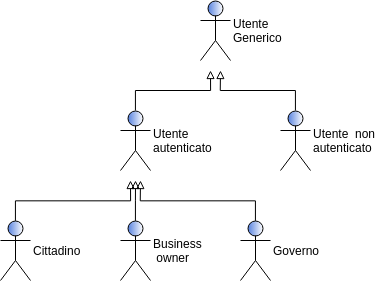
\includegraphics[width=7cm]{res/images/attori_primari.png}
	\centering
	\caption{Gerarchia attori primari}
\end{figure}
\begin{description}[style=nextline]
	\item[Utente Generico]
	Si riferisce ad un utente generico che accede alla piattaforma dal sito web;
	\item[Utente non autenticato]
	Si riferisce ad un utente generico che non ha ancora effettuato l'autenticazione alla piattaforma;
	\item[Proprietario d'azienda] Si riferisce ad un utente non autenticato, proprietario di un'azienda, che potrebbe voler registrare la propria attività sul sistema;
	\item[Utente autenticato]
	Si riferisce ad un utente generico che si è autenticato nel sistema con la procedura di login. Ciò implica che sia in possesso di una chiave pubblica valida sulla rete Ethereum con la quale, precedentemente, ha portato a termine la procedura di autenticazione;
	\item[Cittadino] Si riferisce ad un utente che si è autenticato nel sistema con il ruolo di cliente;
	\item[Azienda] Si riferisce ad un utente che si è autenticato nel sistema con il ruolo di azienda. Le azioni sono eseguite considerando l'azienda come persona giuridica, nonostante le azioni vengano eseguite da un suo rappresentante;
	\item[Governo\glo] Si riferisce ad un utente che si è autenticato al sistema con il ruolo di governo\glo.
\end{description}
\subsubsection{Attori secondari}
\begin{description}[style=nextline]
	\item[MetaMask]
	Plug-in per browser che permette di interfacciarsi con la rete Ethereum\glosp e di validare le transazioni con la propria chiave privata.

\end{description}

\subsection{Elenco dei casi d'uso}
In questa sezione vi sono elencati tutti i casi d'uso individuati. Ogni caso d'uso rappresenta uno scenario per uno o più attori, ovviamente applicabile anche ad eventuali attori derivati. Un singolo caso d'uso inoltre viene esplicato tramite diagrammi dei casi d'uso e possiede una precondizione seguita da una postcondizione.
\begin{figure}[h]
	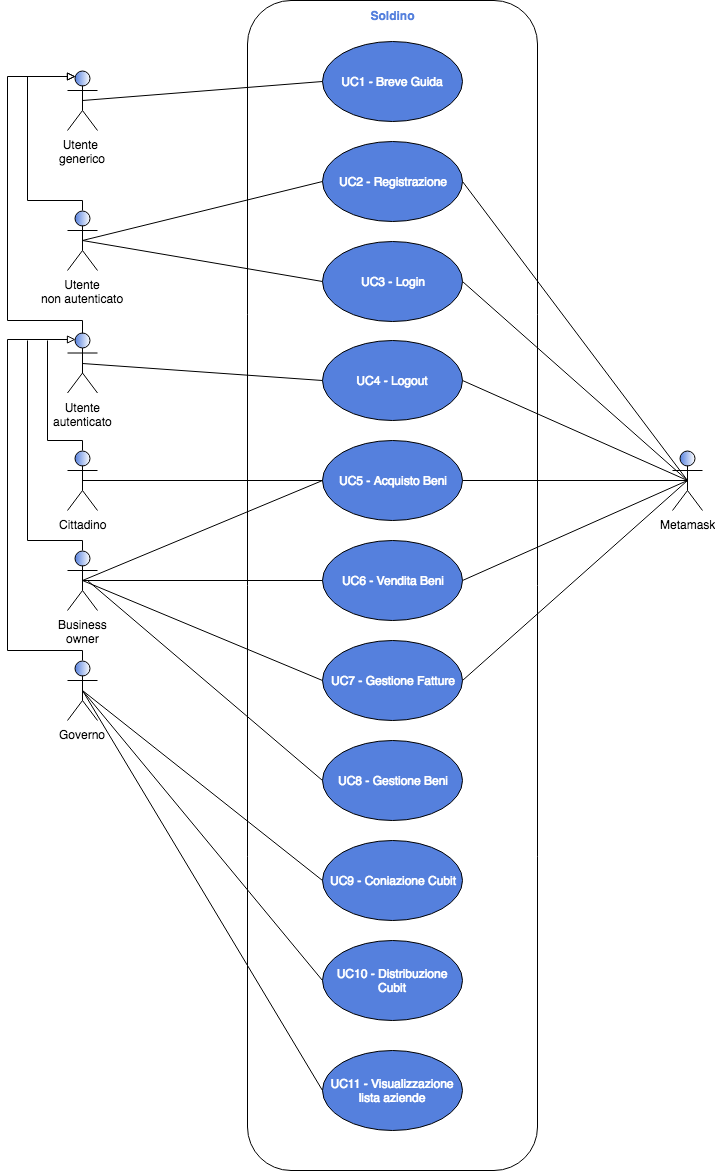
\includegraphics[width=9.38cm]{res/images/Elenco_casi_d_uso.png}
	\centering
	\caption{Elenco dei casi d'uso}
\end{figure}
\subsubsection{UC1 - Breve Guida}
\begin{itemize}
	\item \textbf{Attori Primari}: utente generico;
	\item \textbf{Descrizione}: l'utente visualizza una guida riguardante l'installazione ed il funzionamento del plug-in Metamask\glo. Viene spiegato come impostare le chiavi del plug-in e come utilizzarlo per accedere al sistema;
	\item \textbf{Scenario principale}: l'utente accede alla guida;
	\item \textbf{Precondizione}: il sistema è raggiungibile e funzionante, l'utente desidera ricevere delle informazioni per imparare ad autenticarsi alla piattaforma;
	\item \textbf{Postcondizione}: il sistema fornisce all'utente, attraverso la lettura della guida, tutte le istruzioni necessarie alla registrazione ed all'autenticazione.
	
	
\end{itemize}
\subsubsection{UC2 - Registrazione}
\begin{figure}[h]
	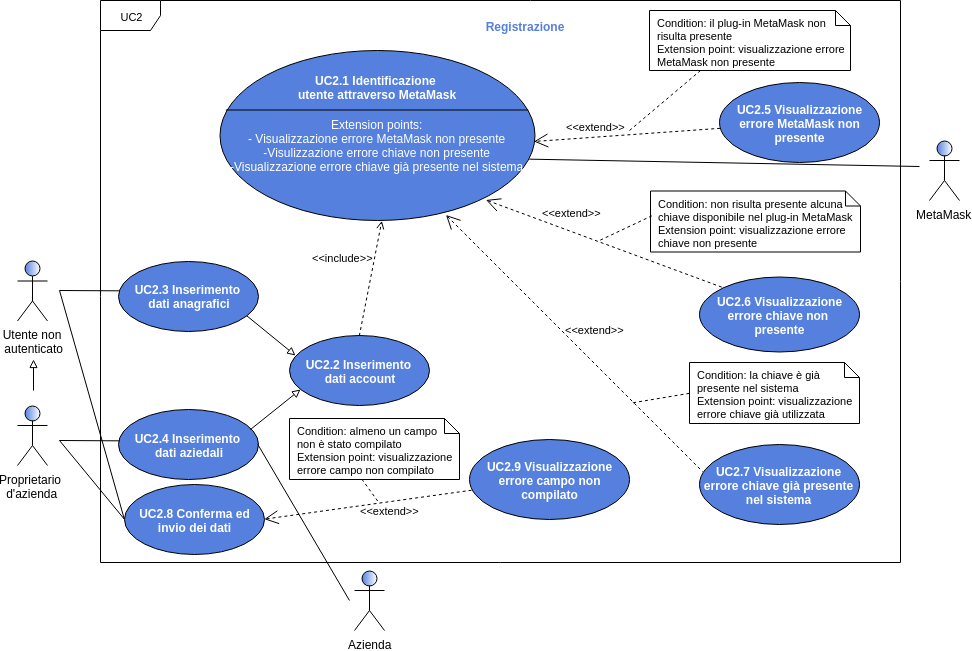
\includegraphics[width=16cm]{res/images/UC2Registrazione.png}
	\centering
	\caption{UC2 - Registrazione}
\end{figure}
\begin{itemize}
	\item \textbf{Attori Primari}: utente non autenticato, eventualmente proprietario d'azienda;
	\item \textbf{Attori Secondari}: MetaMask\glo;
	\item \textbf{Descrizione}: l'utente non autenticato compila tutti i campi richiesti al fine di registrarsi sulla piattaforma, successivamente dovrà aspettare che il proprio account venga verificato da parte del governo\glo;
	\item \textbf{Scenario}: 
	
	\begin{enumerate}[label=\alph*.]
		
		\item l'utente vuole registrarsi come normale \textbf{cittadino}: 
		\begin{enumerate}[label=\roman*.]
			\item l'utente inserisce i dati anagrafici [UC2.3];
			\item l'utente conferma ed invia i dati inseriti [UC2.8].
		\end{enumerate}
	
	
		\item l'utente vuole registrare la propria \textbf{azienda}:
		\begin{enumerate}[label=\roman*.]
			\item l'utente inserisce i dati aziendali [UC2.4];
			\item l'utente conferma ed invia i dati inseriti [UC2.8].
		\end{enumerate}
		

	 
	\end{enumerate}
	\item \textbf{Precondizione}: l'utente ha il plug-in MetaMask\glosp installato e correttamente impostato sul proprio browser, viene considerato dal sistema come un utente non autenticato e desidera registrarsi come cittadino o registrare la propria azienda; 
	\item \textbf{Postcondizione}: il sistema riceve le informazioni dell'utente, le salva ed inoltra la richiesta di verifica ed approvazione al governo\glo.
	
\end{itemize}
\subsubsection{UC2.1 - Identificazione utente attraverso MetaMask\glo}
\begin{itemize}
	\item \textbf{Attori Primari}: utente non autenticato;
	\item \textbf{Attori Secondari}: MetaMask\glo;
	\item \textbf{Descrizione}: il sistema verifica la presenza del plug-in MetaMask\glo, al quale richiede la chiave pubblica che l'utente desidera usare come identificativo e metodo di pagamento. Essendo la chiave univoca, il sistema controlla che nessun utente registrato stia attualmente utilizzandola. Il sistema mostra infine l'interfaccia contente il form di registrazione;
	\item \textbf{Scenario}: il sistema, prima di mostrare il form per la registrazione, controlla la presenza di una chiave\glosp utilizzabile attraverso il plug-in MetaMask\glo.
	\item \textbf{Estensioni}:
		\begin{itemize}
		\item \textbf{UC2.5}: se il plug-in MetaMask\glosp non risulta installato nel browser dell'utente, o è stato disabilitato, esso viene avvisato tramite l'apposito messaggio di errore;
		\item \textbf{UC2.6}: se l'utente non possiede una chiave\glosp su MetaMask\glo, esso viene avvisato tramite l'apposito messaggio di errore;
		\item \textbf{UC2.7}: se è presente una chiave su MetaMask\glo, ma il sistema rileva che essa è già stata utilizzata per la registrazione sulla piattaforma, allora l'utente viene avvisato attraverso l'apposito messaggio di errore.
		\end{itemize}
	\item \textbf{Precondizione}: l'utente ha cliccato sul link per accedere al form di registrazione di un account cittadino o aziendale;
	\item \textbf{Postcondizione}: il sistema ha verificato che la chiave\glosp con la quale l'utente sta cercando di registrarsi non risulti già utilizzata nel sistema. La chiave è salvata e verrà utilizzata durante la registrazione. All'utente è permesso compilare i dati relativi alla tipologia di registrazione richiesta.
	
\end{itemize}
\subsubsection{UC2.2 - Inserimento dati account}
\begin{figure}[h]
	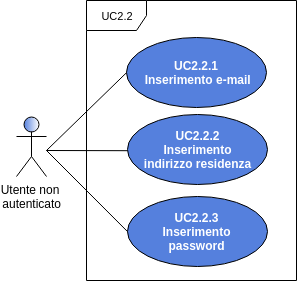
\includegraphics[width=8cm]{res/images/UC2-2RegistrazioneGenerale.png}
	\centering
	\caption{UC2-2 Inserimento dati account}
\end{figure}
\begin{itemize}
	\item \textbf{Attori Primari}: utente non autenticato;
	\item \textbf{Descrizione}: l'utente compila il form contenente i dati relativi all'account;
	\item \textbf{Scenario}: l'utente compila tutti i campi del form riguardanti l'account, ovvero:
		\begin{enumerate}[label=\alph*.]
		\item l'utente inserisce l'email da associare all'account [UC2.2.1];
		\item l'utente inserisce l'indirizzo di residenza da associare all'account [UC2.2.2];
		\item l'utente inserisce la password da associare all'account [UC2.2.3].
		\end{enumerate}
	\item \textbf{Specializzazione}:
	\begin{itemize}
		\item \textbf{UC2.3}: l'utente inserisce i dati relativi alla registrazione di un cittadino;
		\item \textbf{UC2.4}: l'utente inserisce i dati relativi alla registrazione di un'azienda.
	
	\end{itemize}
	\item \textbf{Precondizione}: l'utente ha espresso la volontà di iscriversi alla piattaforma cliccando uno dei link per la registrazione. Il sistema ha rilevato e salvato una chiave\glosp valida attraverso il plug-in MetaMask\glo;
	\item \textbf{Postcondizione}: l'utente ha compilato i campi relativi ai dati dell'account.
	
\end{itemize}
\subsubsection{UC2.2.1 - Inserimento e-mail}
\begin{itemize}
	\item \textbf{Attori Primari}: utente non autenticato;
	\item \textbf{Descrizione}: al fine di portare a termine il processo di registrazione l'utente deve inserire un indirizzo e-mail, campo ritenuto obbligatorio;
	\item \textbf{Scenario}: l'utente compila il campo relativo all'indirizzo e-mail;
	\item \textbf{Precondizione}: il sistema ha reso disponibile il campo per l'inserimento dell'indirizzo e-mail;
	\item \textbf{Postcondizione}: l'utente ha compilato il campo con la propria e-mail.

\end{itemize}
\subsubsection{UC2.2.2 - Inserimento indirizzo di residenza}
\begin{itemize}
	\item \textbf{Attori Primari}: utente non autenticato;
	\item \textbf{Descrizione}: al fine di portare a termine il processo di registrazione l'utente deve inserire un indirizzo di residenza, campo ritenuto obbligatorio;
	\item \textbf{Scenario}: l'utente compila il campo relativo all'indirizzo di residenza;
	\item \textbf{Precondizione}: il sistema ha reso disponibile il campo per l'inserimento dell'indirizzo di residenza;
	\item \textbf{Postcondizione}: l'utente ha compilato il campo con l'indirizzo relativo alla residenza.
\end{itemize}
\subsubsection{UC2.2.3 - Inserimento password}
\begin{itemize}
	\item \textbf{Attori Primari}: utente non autenticato;
	\item \textbf{Descrizione}: al fine di portare a termine il processo di registrazione l'utente deve inserire una password, campo ritenuto obbligatorio;
	\item \textbf{Scenario}: l'utente compila il campo relativo alla password;
	\item \textbf{Precondizione}: il sistema ha reso disponibile il campo per l'inserimento della password;
	\item \textbf{Postcondizione}: l'utente ha compilato il campo con la password scelta.
\end{itemize}
\subsubsection{UC2.3 - Inserimento dati anagrafici}
\begin{figure}[h]
	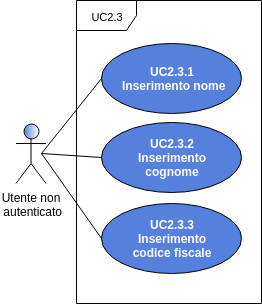
\includegraphics[width=6cm]{res/images/UC2-3Registrazione-cliente.png}
	\centering
	\caption{UC2.3 - Registrazione cittadino}
\end{figure}
\begin{itemize}
	\item \textbf{Attori Primari}: utente non autenticato;
	\item \textbf{Descrizione}: l'utente compila i campi relativi alla registrazione alla piattaforma come cittadino;
	\item \textbf{Scenario}: l'utente ha cliccato sul pulsante di registrazione di un cittadino, il sistema rende disponibile il form di registrazione relativo e l'utente compila tutti i campi necessari;
	\item \textbf{Precondizione}: l'utente ha espresso la volontà di iscriversi alla piattaforma cliccando il link per la registrazione come cittadino. Il sistema ha rilevato e salvato una chiave\glosp valida attraverso il plug-in MetaMask\glo;
	\item \textbf{Postcondizione}: l'utente ha compilato i campi relativi alla registrazione di un cittadino alla piattaforma.
\end{itemize}
\subsubsection{UC2.3.1 - Inserimento nome}
\begin{itemize}
	\item \textbf{Attori Primari}: utente non autenticato;
	\item \textbf{Descrizione}: al fine di portare a termine il processo di registrazione di un nuovo cittadino, l'utente deve inserire il proprio nome;
	\item \textbf{Scenario}: l'utente compila il campo relativo al nome;
	\item \textbf{Precondizione}: il sistema ha reso disponibile il campo per l'inserimento del nome;
	\item \textbf{Postcondizione}: l'utente ha compilato il campo con il proprio nome.
\end{itemize}
\subsubsection{UC2.3.2 - Inserimento cognome}
\begin{itemize}
	\item \textbf{Attori Primari}: utente non autenticato;
	\item \textbf{Descrizione}: al fine di portare a termine il processo di registrazione di un nuovo cittadino, l'utente deve inserire il proprio cognome;
	\item \textbf{Scenario}: l'utente compila il campo relativo al cognome;
	\item \textbf{Precondizione}: il sistema ha reso disponibile il campo per l'inserimento del cognome;
	\item \textbf{Postcondizione}: l'utente ha compilato il campo con il proprio cognome.
\end{itemize}
\subsubsection{UC2.3.3 - Inserimento codice fiscale}
\begin{itemize}
	\item \textbf{Attori Primari}: utente non autenticato;
	\item \textbf{Descrizione}: al fine di portare a termine il processo di registrazione di un nuovo cittadino, l'utente deve inserire il proprio codice fiscale;
	\item \textbf{Scenario}: l'utente compila il campo relativo al codice fiscale;
	\item \textbf{Precondizione}: il sistema ha reso disponibile il campo per l'inserimento del codice fiscale;
	\item \textbf{Postcondizione}: l'utente ha compilato il campo con il proprio codice fiscale.
\end{itemize}
\subsubsection{UC2.4 - Inserimento dati aziendali}
\begin{figure}[h]
	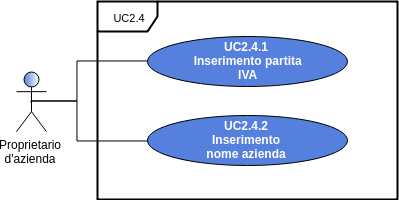
\includegraphics[width=6cm]{res/images/UC2-4RegistrazioneAzienda.png}
	\centering
	\caption{UC2 - Registrazione di un'azienda}
\end{figure}
\begin{itemize}
	\item \textbf{Attori Primari}: proprietario d'azienda;
	\item \textbf{Descrizione}: l'utente compila i campi relativi alla registrazione della propria azienda sulla piattaforma;
	\item \textbf{Scenario}: l'utente ha cliccato sul pulsante di registrazione di un'azienda, il sistema rende disponibile il form di registrazione relativo e l'utente compila tutti i campi necessari;
	\item \textbf{Precondizione}: l'utente ha espresso la volontà di iscriversi alla piattaforma cliccando il link per la registrazione di un'azienda. Il sistema ha rilevato e salvato una chiave\glosp valida attraverso il plug-in MetaMask\glo;
	\item \textbf{Postcondizione}: l'utente ha compilato i campi relativi alla registrazione di un'azienda alla piattaforma.
\end{itemize}
\subsubsection{UC2.4.1 - Inserimento partita IVA}
\begin{itemize}
	\item \textbf{Attori Primari}: proprietario d'azienda;
	\item \textbf{Descrizione}: al fine di portare a termine il processo di registrazione della propria azienda, l'utente deve inserire la relativa partita IVA;
	\item \textbf{Scenario}: l'utente compila il campo relativo alla partita IVA;
	\item \textbf{Precondizione}: il sistema ha reso disponibile il campo per l'inserimento della partita IVA;
	\item \textbf{Postcondizione}: l'utente ha compilato il campo con la partita IVA dell'azienda che intende registrare.
\end{itemize}
\subsubsection{UC2.4.2 - Inserimento nome azienda}
\begin{itemize}
	\item \textbf{Attori Primari}: proprietario d'azienda;
	\item \textbf{Descrizione}: al fine di portare a termine il processo di registrazione della propria azienda, l'utente deve inserire il relativo nome aziendale;
	\item \textbf{Scenario}: l'utente compila il campo relativo al nome aziendale;
	\item \textbf{Precondizione}: il sistema ha reso disponibile il campo per l'inserimento del nome aziendale;
	\item \textbf{Postcondizione}: l'utente ha compilato il campo con il nome dell'azienda che intende registrare.
\end{itemize}



\subsubsection{UC2.5 - Visualizzazione errore MetaMask\glosp non presente}
\begin{itemize}
	\item \textbf{Attori Primari}: utente non autenticato
	\item \textbf{Descrizione}: l'utente visualizza un errore relativo al fatto che non il plug-in MetaMask\glosp non risulta installato o attualmente disabilitato;
	\item \textbf{Scenario}: l'utente non ancora identificato dal sistema tenta di accedere a sezioni che necessitano la presenza di MetaMask\glo, e quest'ultimo non è installato o attualmente disabilitato;
	\item \textbf{Precondizione}: MetaMask\glosp non è presente nel browser dell'utente o è attualmente disabilitato;
	\item \textbf{Postcondizione}: l'utente è a conoscenza che è necessario attivare o installare MetaMask\glosp per proseguire.

\end{itemize}

\subsubsection{UC2.6 - Visualizzazione errore chiave non 
	presente}
\begin{itemize}
	\item \textbf{Attori Primari}: utente non autenticato;
	\item \textbf{Attori Secondari}: MetaMask\glo;
	\item \textbf{Descrizione}:
	l'utente visualizza un messaggio di errore relativo al fatto che non è stata rilevata nessuna chiave\glosp all'interno del plug-in MetaMask\glo;
	\item \textbf{Scenario}: l'utente tenta di accedere ad una sezione del sito che necessita l'identificazione di una chiave\glosp attraverso il plug-in MetaMask\glo, e questo non contiene almeno una chiave\glo;
	\item \textbf{Precondizione}: il plug-in MetaMask\glosp è correttamente configurato, ma non è presente nessuna chiave\glo;
	\item \textbf{Postcondizione}:
	l'utente è consapevole che il plug-in MetaMask\glosp non contiene almeno una chiave\glo.

\end{itemize}




\subsubsection{UC2.7 - Visualizzazione errore chiave già presente nel sistema}
\begin{itemize}
	\item \textbf{Attori Primari}: utente non autenticato;
	\item \textbf{Attori Secondari}: MetaMask\glo;
	\item \textbf{Descrizione}:
	l'utente visualizza un messaggio di errore relativo al fatto che la chiave\glosp prelevata dal plug-in MetaMask\glosp risulta già presente nella piattaforma;
	\item \textbf{Scenario}: l'utente tenta di registrarsi al sito utilizzando una chiave\glosp già presente nel sistema;
	\item \textbf{Precondizione}: MetaMask\glosp è correttamente configurato, ma la chiave\glosp selezionata nel plug-in è già stata utilizzata nella piattaforma;
	\item \textbf{Postcondizione}:
	l'utente è consapevole che la chiave\glosp selezionata nel plug-in MetaMask\glosp è già stata utilizzata nella piattaforma, e quindi che necessita di un'altra chiave per effettuare la nuova registrazione.
\end{itemize}

\subsubsection{UC2.8 - Conferma ed invio dei dati}
\begin{itemize}
	\item \textbf{Attori Primari}: utente non autenticato, eventualmente proprietario d'azienda;
	\item \textbf{Descrizione}:
	l'utente preme il pulsante per la conferma e l'invio dei dati. A schermo viene mostrato un messaggio che conferma il successo dell'operazione e spiega di attendere la verifica da parte del governo\glosp prima di poter effettivamente accedere alla piattaforma.
	\item \textbf{Scenario}: l'utente preme il pulsante di verifica ed invio dei dati dopo aver compilato i campi del form;
	\item \textbf{Estensioni}: 
	\begin{itemize}
		\item \textbf{UC2.9}: l'utente preme il pulsante di verifica senza aver compilato almeno uno dei campi del form, viene visualizzato il relativo errore;
	\end{itemize}
	\item \textbf{Precondizione}: il sistema permette all'utente di compilare il form di registrazione. \`E presente il pulsante per la conferma dei dati;
	\item \textbf{Postcondizione}:
	l'utente è consapevole che la richiesta di registrazione è avvenuta con successo ed è consapevole del fatto che dovrà attendere la verifica dell'account da parte del governo\glo.
\end{itemize}

\subsubsection{UC2.9 - Visualizzazione errore campo non compilato}
\begin{itemize}
	\item \textbf{Attori Primari}: utente non autenticato;
	\item \textbf{Descrizione}:
	l'utente visualizza un messaggio di errore relativo al fatto che almeno uno dei campi del form di registrazione risulta non compilato;
	\item \textbf{Scenario}: l'utente tenta di confermare i dati della registrazione senza aver compilato tutti i dati del form;
	\item \textbf{Precondizione}: il sistema permette all'utente di compilare il form di registrazione. \`E presente il pulsante per la conferma dei dati;
	\item \textbf{Postcondizione}:
	l'utente è consapevole che per inviare i dati e terminare la procedura di registrazione deve compilare tutti i campi presenti nel form.
\end{itemize}








\subsubsection{UC3 - Login}
\begin{figure}[h]
	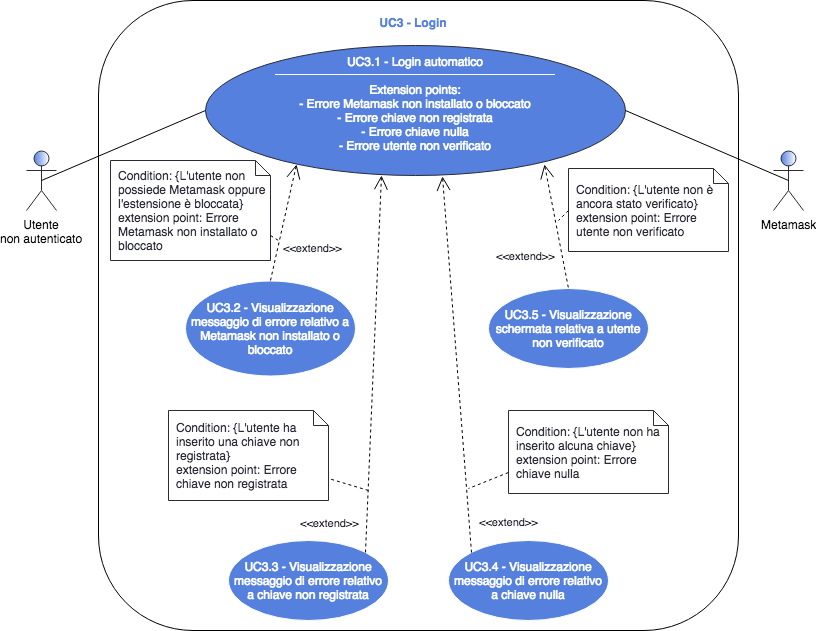
\includegraphics[width=10.5cm]{res/images/UC3Login.png} %da adattare in larghezza
	\centering
	\caption{UC3 - Login}
	
\end{figure}
\begin{itemize}
	\item \textbf{Attori Primari}:
	utente non autenticato;
	\item \textbf{Attori Secondari}:
	MetaMask\glo;
	\item \textbf{Descrizione}:
	l'utente prova a farsi identificare tramite l'interfaccia web per mezzo di MetaMask\glo;
	\item \textbf{Scenario}:
	l'utente non è identificato dal sito ed esegue il login;
	\item \textbf{Precondizione}:
	l'utente non è identificato dalla piattaforma web;
	\item \textbf{Postcondizione}:
	l'utente è identificato dalla piattaforma web. 
\end{itemize}
\subsubsection{UC3.1 - Login automatico}
\begin{itemize}
	\item \textbf{Attori Primari}:
	utente non autenticato;
	\item \textbf{Attori Secondari}:
	MetaMask\glo;
	\item \textbf{Descrizione}:
	in modo automatico, il sistema procede all'identificazione dell'utente;
	\item \textbf{Scenario}:
	l'utente non ancora autenticato richiede il login;
	\item \textbf{Estensioni}:
	\begin{itemize}
		\item \textbf{UC2.5}: se l'utente non dispone di MetaMask o ha disabilitato l'estensione, viene visualizzato un messaggio di errore a riguardo;
		\item \textbf{UC2.6}: se l'utente non possiede una chiave\glosp su MetaMask\glo, esso viene avvisato tramite l'apposito messaggio di errore;
		\item \textbf{UC3.2}: se l'utente tenta di accedere al sito tramite MetaMask senza aver mai provveduto a registrarsi, riceverà un messaggio di errore a riguardo;
		\item \textbf{UC3.3}: se l'utente si è registarto sul sito da poco ma non gli è ancora stato validato l'account, visualizzerà un messaggio di errore a riguardo.
	\end{itemize}
	\item \textbf{Precondizione}:
	l'utente richiede alla piattaforma di venire identificato;
	\item \textbf{Postcondizione}:
	tramite il plugin MetaMask\glo l'utente viene riconosciuto.
\end{itemize}
\subsubsection{UC3.2 - Visualizzazione messaggio di errore relativo a chiave non registrata}
\begin{itemize}
	\item \textbf{Attori Primari}:
	utente non autenticato;
	\item \textbf{Descrizione}:
	l'utente visualizza un messaggio di errore dovuto al fatto che ha tentato il login senza essersi registrato in precedenza;
	\item \textbf{Scenario}:
	l'utente tenta il login alla piattaforma senza aver effettuato la registrazione;
	\item \textbf{Precondizione}:
	l'utente richiede l'accesso al sito;
	\item \textbf{Postcondizione}:
	l'utente è consapevole di dover registrarsi per poter poi accedere.
\end{itemize}
\subsubsection{UC3.3 - Visualizzazione schermata relativa a utente non verificato}
\begin{itemize}
	\item \textbf{Attori Primari}:
	utente non autenticato;
	\item \textbf{Descrizione}:
	l'utente visualizza una schermata che esplica il fatto che il proprio account non è ancora stato verificato in seguito alla registrazione;
	\item \textbf{Scenario}:
	l'utente registrato da non molto tenta il login ma la richiesta viene rigettata, in quanto è a disposizione di un account non ancora validato;
	\item \textbf{Precondizione}:
	l'utente richiede il login alla piattaforma;
	\item \textbf{Postcondizione}: l'utente sa che dovrà attendere la validazione del propio account prima di procedere con il prossimo login.
\end{itemize}
\subsubsection{UC4 - Logout}
\begin{figure}[h]
	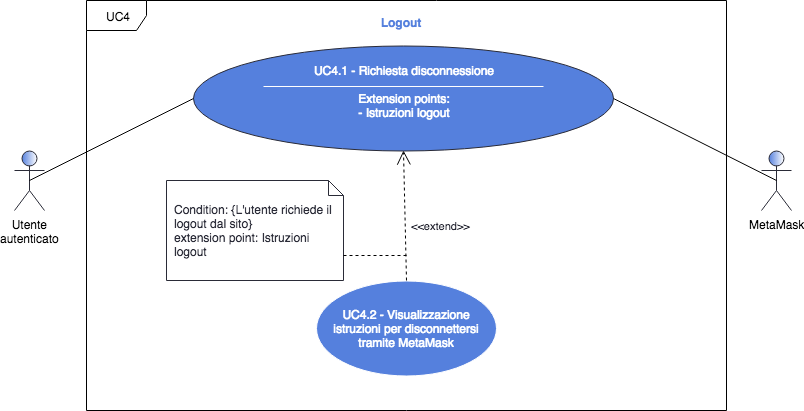
\includegraphics[width=15.5cm]{res/images/UC4Logout.png} %da adattare in larghezza
	\centering
	\caption{UC4 - Logout}
	
\end{figure}
\begin{itemize}
	\item \textbf{Attori Primari}:
	utente autenticato;
	\item \textbf{Attori Secondari}:
	MetaMask\glo;
	\item \textbf{Descrizione}: l'utente richiede il logout dalla piattaforma web ed effettua ciò tramite MetaMask\glo;
	\item \textbf{Scenario}: l'utente è identificato dal sito ed esegue il logout.
	\item \textbf{Precondizione}: l'utente è identificato dalla piattaforma web e richiede di essere disconnesso dal sito;
	\item \textbf{Postcondizione}: vengono fornite le istruzioni necessarie per affrontare il Logout tramite MetaMask\glo. 
\end{itemize}
\subsubsection{UC4.1 - Richiesta disconnessione}
\begin{itemize}
	\item \textbf{Attori Primari}:
	utente autenticato;
	\item \textbf{Attori Secondari}:
	MetaMask\glo;
	\item \textbf{Descrizione}: l'utente clicca sul bottone dedicato al logout e si appresta a leggere le istruzioni per farlo tramite MetaMask\glo;
	\item \textbf{Scenario}: l'utente richiede la disconnessione dalla piattaforma web;
	\item \textbf{Estensioni}:
	\begin{itemize}
		\item \textbf{UC4.2}: al conseguimento della richiesta di logout, l'utente riceve informazioni sul da farsi per procedere a completare ciò;
	\end{itemize}
	\item \textbf{Precondizione}: l'utente autenticato dal sistema non ha idea di come disconnettersi dal sito;
	\item \textbf{Postcondizione}: l'utente può visualizzare il modo corretto per eseguire la disconnessione dalla piattaforma.
	
\end{itemize}
\subsubsection{UC4.2 - Visualizzazione istruzioni per disconnettersi tramite MetaMask\glo}
\begin{itemize}
	\item \textbf{Attori Primari}:
	utente autenticato;
	\item \textbf{Attori Secondari}:
	MetaMask\glo;
	\item \textbf{Descrizione}: l'utente visualizza le istruzioni per procedere al logout tramite MetaMask\glo;
	\item \textbf{Scenario}: in seguito alla richiesta di disconnessione, l'utente riceve le informazioni necessarie per effettuare tale operazione;
	\item \textbf{Precondizione}:l 'utente non ha idea di come disconnettersi tramite MetaMask\glo;
	\item \textbf{Postcondizione}: l'utente ha le abilità necessarie al conseguimento di un logout eseguito in modo corretto e sicuro tramite il plugin MetaMask\glo.
\end{itemize}

\subsubsection{UC5 - Acquisto Beni}
\begin{itemize}
	\item \textbf{Attori Primari}:
	\item \textbf{Descrizione}:
	\item \textbf{Scenario}:
	\item \textbf{Precondizione}:
	\item \textbf{Postcondizione}:
\end{itemize}
\subsubsection{UC6 - Vendita Beni}
\begin{itemize}
	\item \textbf{Attori Primari}:
	\item \textbf{Descrizione}:
	\item \textbf{Scenario}:
	\item \textbf{Precondizione}:
	\item \textbf{Postcondizione}:
\end{itemize}
\subsubsection{UC7 - Gestione Fatture}
\begin{itemize}
	\item \textbf{Attori Primari}:
	\item \textbf{Descrizione}:
	\item \textbf{Scenario}:
	\item \textbf{Precondizione}:
	\item \textbf{Postcondizione}:
\end{itemize}
\subsubsection{UC8 - Gestione Beni}
\begin{itemize}
	\item \textbf{Attori Primari}:
	\item \textbf{Descrizione}:
	\item \textbf{Scenario}:
	\item \textbf{Precondizione}:
	\item \textbf{Postcondizione}:
\end{itemize}
\subsubsection{UC9 - Coniazione Cubit}
\begin{itemize}
	\item \textbf{Attori Primari}: governo;
	\item \textbf{Descrizione}: viene coniata una quantità definita di Cubit\glo;
	\item \textbf{Scenario}: il governo ritiene necessario coniare ulteriori Cubit\glo rispetto a quelli attualmente presenti sul mercato;
	\item \textbf{Precondizione}: siano \texttt{x} i Cubit\glo che il governo vuole coniare e \texttt{n} i Cubit\glo attualmente in circolo;
	\item \textbf{Postcondizione}: i Cubit\glo in circolo sono \texttt{n+x}.
\end{itemize}
\subsubsection{UC10 - Distribuzione Cubit}
\begin{itemize}
	\item \textbf{Attori Primari}: governo;
	\item \textbf{Attori Secondari}: cittadino, business owner;
	\item \textbf{Descrizione}: uno o più  utenti, che siano essi cittadini o business owners, riceveno una quantità di Cubit\glo da parte del governo;
	\item \textbf{Scenario}: il governo clicca sull'apposito pulsante per distribuire una somma di Cubit definita, ad una o più persone specificate; 
	\item \textbf{Precondizione}: il governo viene notificato di dover distribuire una quantità specifica di Cubit\glo ad uno o più utenti specifici;
	\item \textbf{Postcondizione}: tali utenti ricevono i Cubit\glo da parte del governo.
\end{itemize}
\subsubsection{UC11 - Visualizzazione lista aziende}
\begin{figure}[h]
	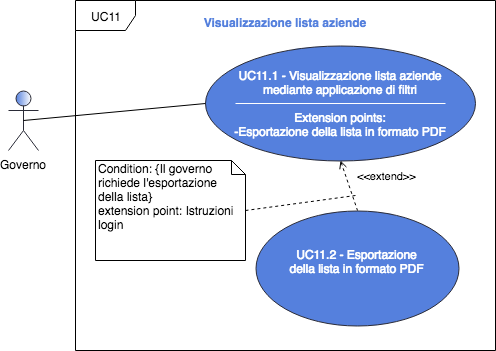
\includegraphics[width=10.5cm]{res/images/UC11Visualizzazione.png} %da adattare in larghezza
	\centering
	\caption{UC12 - Validazione nuovo account registrato}
	
\end{figure}
\begin{itemize}
	\item \textbf{Attori Primari}: governo;
	\item \textbf{Descrizione}: il governo può vedere una lista dettagliata relativa alle aziende che hanno pagato o che devono ancora pagare per uno specifico trimestre;
	\item \textbf{Scenario}: il governo richiede la lista delle aziende;
	\item \textbf{Precondizione}: il governo non è in possesso di alcuna lista;
	\item \textbf{Postcondizione}: il governo è in possesso di ciò che ha richiesto.
\end{itemize}
\subsubsection{UC11.1 - Visualizzazione lista aziende mediante l'applicazione di filtri}
\begin{itemize}
	\item \textbf{Attori Primari}: governo;
	\item \textbf{Descrizione}: il governo può vedere una lista dettagliata in base ai filtri applicati ;
	\item \textbf{Scenario}: il governo richiede la lista ad hoc delle aziende;
		\item \textbf{Estensioni}:
	\begin{itemize}
		\item \textbf{UC11.2}: in seguito alla richiesta di esportazione della lista precedentemente creata ad hoc, il governo può ottonere tale file;
	\end{itemize}
	\item \textbf{Precondizione}: il governo non dispone della lista personalizzata delle aziende ed applica alcuni filtri nell'apposita sezione del sito;
	\item \textbf{Postcondizione}: il governo è in possesso di una lista personalizzata secondo le proprie esigenze.
\end{itemize}
\subsubsection{UC11.2 - Esportazione della lista in formato PDF}
\begin{itemize}
	\item \textbf{Attori Primari}: governo;
	\item \textbf{Descrizione}: il governo ottiene in formato PDF la lista precedentemente creata;
	\item \textbf{Scenario}: il governo clicca sull'apposito pulsante per esportare la lista in PDF;
	\item \textbf{Precondizione}: il governo ha ottenuto una lista secondo alcuni filtri e non è in possesso della versione PDF, pertanto clicca sull'apposito pulsante;
	\item \textbf{Postcondizione}: il governo ora è in possesso della versione PDF della lista precedentemente filtrata.
\end{itemize}
\subsubsection{UC12 - Validazione nuovo account registrato}
\begin{figure}[h]
	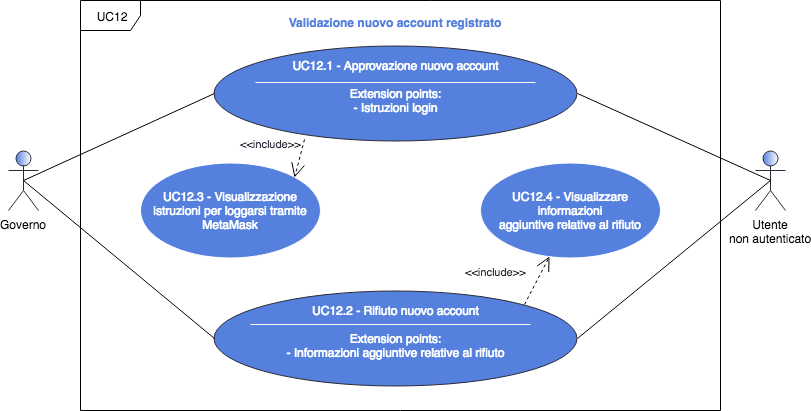
\includegraphics[width=15.5cm]{res/images/UC12Validazione.png} %da adattare in larghezza
	\centering
	\caption{UC12 - Validazione nuovo account registrato}
	
\end{figure}
\begin{itemize}
	\item \textbf{Attori Primari}:
	governo;
	\item \textbf{Attori Secondari}:
	utente non autenticato;
	\item \textbf{Descrizione}: l'account utente può venire rigettato o approvato dal governo;
	\item \textbf{Scenario}: l'utente si è registrato da poco ed attente una risposta da parte del governo in merito alla validazione del proprio account;
	\item \textbf{Precondizione}: l'utente è in coda di attesa per la validazione dell'account;
	\item \textbf{Postcondizione}: l'account utente viene approvato o rigettato. 
\end{itemize}
\subsubsection{UC12.1 - Approvazione nuovo account}
\begin{itemize}
	\item \textbf{Attori Primari}:
	governo;
	\item \textbf{Attori Secondari}:
	utente non autenticato;
	\item \textbf{Descrizione}: l'account utente viene approvato;
	\item \textbf{Scenario}: in seguito alla registrazione, il governo riconosce validi i dati immessi dall'utente;
	\item \textbf{Estensioni}:
	\begin{itemize}
		\item \textbf{UC12.3}: in seguito all'approvazione dell'account, l'utente visualizza una breve e concisa guida su come loggarsi al sito;
	\end{itemize}
	\item \textbf{Precondizione}: l'utente non ha i permessi per loggarsi al sito;
	\item \textbf{Postcondizione}: l'utente può visualizzare il modo corretto per eseguire il login alla piattaforma.
	
\end{itemize}
\subsubsection{UC12.2 - Rifiuto nuovo account}
\begin{itemize}
	\item \textbf{Attori Primari}:
	governo;
	\item \textbf{Attori Secondari}:
	utente non autenticato;
	\item \textbf{Descrizione}: l'account utente viene rifiutato;
	\item \textbf{Scenario}: in seguito alla registrazione, il governo riconosce non validi i dati immessi dall'utente;
	\item \textbf{Estensioni}:
	\begin{itemize}
		\item \textbf{UC12.4}: in seguito al rigetto  dell'account, l'utente visualizza dettagli aggiuntivi del perchè non è stato accettato;
	\end{itemize}
	\item \textbf{Precondizione}: l'utente è in attesa di approvazione;
	\item \textbf{Postcondizione}: l'utente può visualizzare ulteriori dettagli in seguito al rifiuto dell'approvazione di validità proprio account.
	
\end{itemize}
\subsubsection{UC12.3 - Visualizzazione istruzioni per loggarsi tramite MetaMask\glo}
\begin{itemize}
	\item \textbf{Attori Primari}:
	governo;
	\item \textbf{Attori Secondari}:
	utente non autenticato;
	\item \textbf{Descrizione}: l'utente visualizza le istruzioni per procedere al login tramite MetaMask\glo;
	\item \textbf{Scenario}: in seguito all'approvazione dell'account, l'utente riceve le informazioni necessarie per effettuare tale operazione;
	\item \textbf{Precondizione}:l 'utente non ha idea di come connettersi tramite MetaMask\glo;
	\item \textbf{Postcondizione}: l'utente ha le abilità necessarie al conseguimento di un login eseguito in modo corretto e sicuro tramite il plugin MetaMask\glo.
\end{itemize}
\subsubsection{UC12.4 - Visualizzazione informazioni aggiuntive in merito al rigetto dell'account}
\begin{itemize}
	\item \textbf{Attori Primari}:
	governo;
	\item \textbf{Attori Secondari}:
	utente non autenticato;
	\item \textbf{Descrizione}: l'utente visualizza le informazioni aggiuntive relative al rigetto del proprio account;
	\item \textbf{Scenario}: in seguito al rifiuto dell'account, l'utente riceve le informazioni relative a tale rigetto da parte del governo;
	\item \textbf{Precondizione}:l 'utente non ha idea del perchè non è stato accettato;
	\item \textbf{Postcondizione}: l'utente riconosce di aver inserito dati falsi o contenenti errori, pertanto dovrà riprovare la registrazione.
\end{itemize}